\documentclass[10pt,twocolumn]{extarticle}
\usepackage{graphicx}
\usepackage[a4paper, margin=2cm, footskip=0.25in]{geometry}
\usepackage{url}
\usepackage{tabularx}
\usepackage{longtable}
\usepackage{hyperref}
\usepackage{titling}
\usepackage[backend=bibtex,style=numeric-comp,sorting=none]{biblatex}
\usepackage{booktabs}
\usepackage{multicol}
\usepackage{float}
\usepackage{multirow}
\usepackage{xcolor}
\usepackage{colortbl}
\usepackage{tabulary}
\usepackage{listings}
\usepackage{amsmath}
\usepackage{booktabs}
\usepackage{cleveref}
\usepackage{array}
\usepackage{subcaption}
\usepackage{tabularx}

% Define the geometry of the page
\geometry{a4paper, left=20mm, right=20mm, top=20mm, bottom=20mm}

% Customize the sections
%\title{}
%\titleformat{\subsection}[block]{\bfseries\large}{\thesubsection}{1em}{}

% Customize captions
\captionsetup{font=small, labelfont=bf}
\addbibresource{refs.bib} 
% Set citation style to numbered
%\setcitestyle{numbers}

% Document title and author
\title{Attack.}
\author{Udesh Habaraduwa}
\date{\today}

\begin{document}

\maketitle

\begin{abstract}
% A friend of mine, Kagach Mark, asked at some point how one might approach \textit{cognitive work} like an professinal athelete. The question struck me and has stuck with me for several months. Thus, I first tried to understand what that the comparison was. What does it mean to be a \textit{professional athelete} and how would you translate that to maximizing the amount of productive work I can engage in over the course of my life? In what follows, I present not a detailed thesis on this topic (though I will include references where possible) but a distillation of how I generally live my life. I do not claim that this answers Marks's question, nor that I am a professional, only that I believe 

It can be difficult to come up with a reasonable structure fo one's life. The space of possible ways of behaving is essentially unbounded (subject to biology and physics). Herein I outline my structure which I have developed to help me lead a productive life that I can be proud of. It outline the structure of my day, starting from waking to going back to bed. My hope is that it may be useful as an (initial) template, to be modified as needed, when one is first attempting to engineer one's life in a conscious manner, aiming at accumulating hours of productive time. I find that leisure is empty without the grind. If you find this to be the case, perhaps this will be useful. 

\end{abstract}

\section{Introduction}
In this document, I will outline the various aspects of my life that contribute to my productivity. These include daily routines, practices I follow, plans I make, and the mental frameworks I use to approach tasks and challenges. It will be interspersed with (potentially valuable) wisdom where appropriate. Otherwise, it will be a concrete description of the different parts of my daily life. Let me state at the outset that this is not for everyone. Not everyone should or want to live like this. Note also that much of this is a post-hoc analysis of the behavior model as it now stands, not a recounting of a grand plan that I put into action. I made many, many mistakes along the way. Everyone has to start somewhere and what follows is an analysis of where I am now. If you find something here that is ``a waste of time'', please reach out to me (preferably with evidence). 
%  Note also that I prefer to use some specific machine learning (ML) / mathetical terms and formalisms where I can. This is not to make this ``sound cool'' but it is an attempt to force myself to be as precise as possible. It is also quite fun. 

% First, let me try to formalize what I'm saying for the sake of showing that there is a measure that I am looking at which influences my decisions. The function ($f$) to be optimized is the \textit{productive output} and the model which I describe herein has served me relatively well acheiving stasifying results. At the time of writing, the performance of $f$ is quantified using \textit{grade point average} (GPA) as a heusristic measure (for understanding) and \textit{quality} of work generated (for generation). The later is subjective (though many were generated in the service of graded assignments) and acessed through a self evaluation (comparing myself to myself yesterday) as well as feedback from accomplished academics. For example, if a piece of work has potential to be published (as a function of novelty and significance of results) as indicated by a supervisor, this is concsidered a strong positive signal. Actions have been optimized to move in the direction of increasing these signals.

% If I was to name the primary determiner of the output of $f$, it would be \textit{time spent working} (let total time alive be the function $t_{max}$ and work be $t_{work}$) such that $f\rightarrow f(t_{work})$. Indeed, I find $t_{max}$ to be the only real resource that everyone is born with and it flows of its own accord. If given enough time ($t_{work} \rightarrow\infty$), even a sub-optimal model (assuming $f > 0$ ) will generate a net positive accumulation of results.  However, we do not have $\infty$ time to live or work. Thus, I am also interested in \textit{maximizing the area under the curve} of $t_{work}$. That is, of all the time I have left to live, I want to model behavior such that I can spend my time maximally engaged in productive work under the assumption that I have approxiamtely 80 years to life (50 more years at the time of writing). Importantly, and perhaps fortunately, given the type of work I want to be engaged in (i.e., science) this ammounts to \textit{}

First, I do not believe that physical and cognitive decline as you age is inevitable. As the Buddha recognized, the fundamental cause of suffering is ignorance. I take this to mean \textit{the lack of knowledge} and that if something does not violate the laws of physics, it is simply a matter of figuring out how to do it (refer works by David Deutsch \cite{deutsch2011beginning}). With that being said, I recognize that at the time of writing, this decline is very likely. Thus, the structure of my life is broadly guided by following:

\begin{enumerate}
    \item Of the time I have left to live, I want to maximize the time I am able to live independently (e.g., go to the grocery store, pick up weights etc.).
    \subitem This guides my approach to structuring how I exercise.
    \item I want to maximize the time I can spend being useful to humanity (i.e., be cognitively functional).
    \subitem This guides my approach to how I structure my working and social life.
\end{enumerate}

That being said, I find that the structure of my life has the following attributes:

\begin{itemize}
    \item \textit{Robust} to changes in the environment (e.g., having to work in unexpected places).
    \item \textit{Degrades gracefully} in the face of unexpected shocks (e.g., sickness, family emergencies) such that productivity does not plummet to zero for large stretches of time.
    \item \textit{Accommodates social interaction} to a satisfying degree.
    \item \textit{Salable} at times when I have to work more or less (e.g., around deadlines, social holidays)
\end{itemize}


I have found the following points of leverage (in no specific order) as targets:
\begin{enumerate}
    \item Sleep
    \item Exercise
    \item Meditation
    \item Diet (including supplementation)
\end{enumerate}

\subsection{Disclaimer} 

Finally, let me state that I am not an expert and I do not play one on the internet. Thus, let me state my biases clearly. My primary sources of information in this space is podcasts and specific people. They are as follows: 

\begin{enumerate}
    \item \textbf{Longetivity and general health :}
    \subitem Peter Attia
    \subitem Rhonda Patrick 
    \subitem Andrew Huberman 
    \item \textbf{Training, nutrition, and performance :}
    \subitem Layne Norton
    \subitem Andy Galpin 
    \item \textbf{Philosophy and Psychology}
    \subitem Ryan Holiday (and the stoics)
    \subitem Jordan Peterson
    \subitem Carl Jung
    \subitem David Deutsch
    \subitem Steven Pinker
    \subitem (honoroable mention) My parents 
\end{enumerate}

I outline my general operating manual as it stands at the time of writing and is subject to change (as it should). I do not claim to follow everything to the letter everyday, I aim for living in this way at least 80-90\% of the time. I only write this to serve as useful document to share with people as I get asked many of these questions routinely. 

\subsection{Why don't I read all the research myself ?}

Though in what follows I have cited research where appropriate, especially in diet and fitness cases, you will find that I often link to videos and blog posts from the above sources. It's fair to ask why I should trust these sources.

Firstly, the space of research is vast. Most of these sources have entire teams that are dedicated to sifting through research papers. Secondly, it takes time and training to be able to properly evaluate the results of a study. Just because one study shows one effect (or lack there of) does not mean that there is a signal there. Studies are conducted under a variety of constraints (e.g., time and money) and thus have to make methodological decisions (e.g., what to measure and what statistical tests to use) that may or may not be appropriate. Without properly understanding the mechanisms of glucose metabolism, how can I can evaluate one study done in a specific group of people at a specific time ? The right questions to ask will likely not even occur to me.

Therefore, I rely on these sources because over years of following their work, I have tried many of the things they suggest and have found tangible benefits. Over years of engaging with their content, I have come to find that they are less likely to be dogmatic in their positions, have the necessary resources to invest in research, and the appropriate training to understand the material. All that being said, we are all different from our genes on up and your mileage may vary. 

\section{Know thy self}
A brief aside to mention a couple of things that I believe have been very useful to me over the past 3-5 years. 

I highly recommend first understanding your personality \cite{understandmyself2024}. While factor analytic methods like the Big-Five scale (and IQ) have come under intense scrutiny of late \cite{feher2021looking}, I have found the results personally useful. It added some color and context to my perception of myself, on top of the empirical evidence showing the association of the traits with a variety of outcomes (e.g., leadership style \cite{judge2000five} and relationship satisfaction \cite{o2019big}). 

Secondly, I recommend taking a structured approach to generating a (blurry) vision for your future along with a (tentative) plan to get there. I used \cite{selfauthoring} which is backed with empirical support for its efficacy in improving long to medium term outcomes \cite{morisano2010setting,schippers2015scalable}. A very rough idea of this process (with my own addition of the habits part) is visualized in figure \ref{fig:decompose}. For a brief description of this process, refer section \ref{sec:decomposing} in the appendix. Based on the intervention used by \cite{schippers2015scalable}, I have created a shorter version (titled Goal Setting) (for the future authoring portion) which can be found here \url{https://github.com/onedeeper/miscStuffToShare/tree/main}.

Finally, in the vein of finding what to work on and thinking about how you want your life to turn out, I recommend Paul Graham's essays \cite{graham_essays}, specifically ``How To Do Great Work''.

\begin{figure*}[htbp]
    \centering
    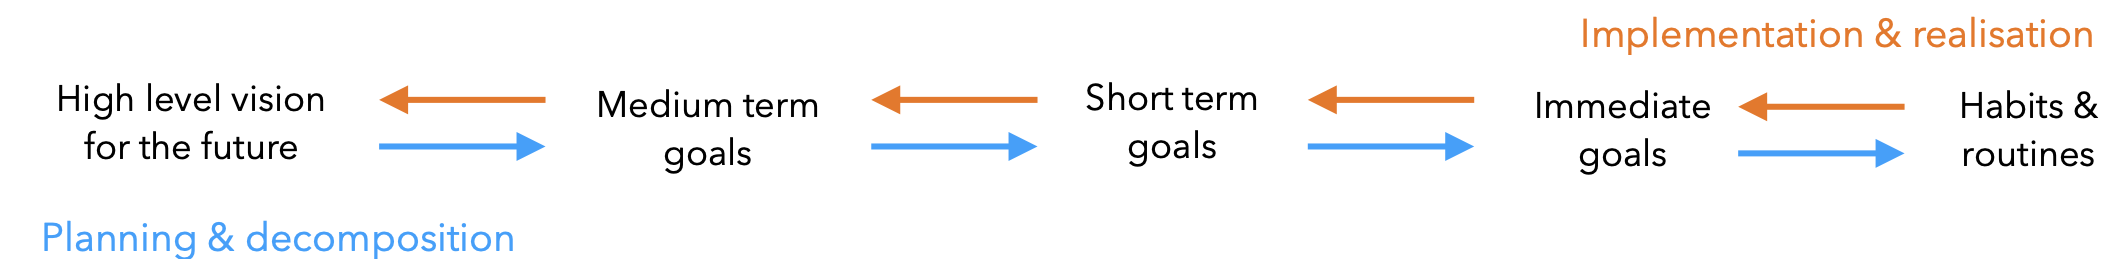
\includegraphics[scale=0.4]{decompose.png}
    \caption{Going from vision to habits}
    \label{fig:decompose}
  \end{figure*}

\section{Daily Routines}
This section outlines my attempt to optimize factors 1-4 identified in the previous section. I do not try to convince you of anything though I will provide relevant sources which can be consulted for further details.

To begin, I spend most of day in a ``fasted'' state : meaning I do not consume calories until all of the work for the day is done or. It serves as bright border around my day such that once it's done, I am able to temporarily silence the voice in my head that impels me to work. I also find that not having to think about food for a big chunk of my day frees up my mind (more in section \ref{sec:diet}).

\subsection{Morning Routine}

The following is my morning routine. I follow it most days of my life, regardless of where I am, what I'm doing, or who I'm with.
\begin{itemize}
    \item \textit{Wake up at (approximately) the same time every day} : Circadian rhythm (the day-night cycle) plays a pivotal role in a range of bodily functions, from insulin response \cite{boden1996evidence} to alertness \cite{dijk1992circadian}. I try to keep this as regular as possible (through weekends and holidays) though sometimes I turn off my morning alarm before bed. For example, I might much rather get the benefits of being more rested than waking up on schedule (e.g., I got home unexpectedly late or had to eat later than usual). Here I'm assuming that the benefit of adequate hours of sleep outweighs the gain from waking up on schedule. This happens only occasionally and not enough to disrupt my rhythm. I usually wake up at the same time anyways but I give my body the option of taking as long as it needs.
    \item \textit{Meditate} : This has been a long standing practice of mine. For me, it provides a strong grounding for the day. It sets the tone so to speak. The neuroscience field has recently taken an interest in this time honored tradition \cite{tang2015neuroscience} and appears to be a common factor amongst many highly productive people \cite{ferriss2018}. I practice a very basic form of focused\-attention mindfulness meditation \cite{analayo2019meditation} for 20 minutes. I try to focus on the movement of air in and out of my nostrils. Many flavors exist from a variety of  (free or paid) sources \cite{tenpercenthappier,calm,headspace}. I am a fan of Waking Up\cite{wakingup} and I find it to be an excellent starting point. Additionally, the creators graciously give you access to the app for free if you ask for it (see \textit{scholarship} on the linked page).
    \item \textit{Begin first work session} : I begin my first 90 minute work session (described more in section \ref{sec:productive_pracs}). This is not designed to be a heavy lift. Ideally this continues from a point that I was making progress on at the conclusion of the previous day. That is, I already know what needs to get done and where I'm going (e.g., I've got the outline of a piece of code in place and I just need to fill in the syntax). If I don't have something that I can get rolling easily from the previous day, I look to tasks that are not very demanding but need to be done regardless (this could be scheduling meetings, checking e-mail, skimming some abstracts of papers). This session basically acts as a warm-up. 
    \item \textit{Coffee or tea} : This is usually my first and only ingestion of caffeine in the day. It is consumed without milk or sugar. It happens approximately 90 minutes after I wake up (approximately 45 minutes into my first work session). Caffeine has a storied history \cite{weinberg2004world} and has shown efficacy in improving cognitive \cite{jarvis1993does} and physical performance \cite{jimenez2021caffeinated,hubermancaffeine}.
    \item \textit{Morning sunlight} : At the conclusion of my first session, I go outside to get sunlight in my eyes (weekends, before more work sessions) or shower and head out for the day (weekdays). This is to regulate my circadian rythm \cite{blume2019effects}. Ideally I would do this first thing in the morning but it is adjusted to make an allowance for the late sunrises during winter months. 
    \item \textit{Cold shower} : I finish off my morning routine with a short cold shower (as cold as I can get from the shower head). While long exposures and complete submersion has shown to induce significant increases in dopamine levels \cite{vsramek2000human}, it's unlikely a short shower has the same effect. None the less, it is uncomfortable and I never want to do it, which is why I do it. When available, I do use a cold plunge.
\end{itemize}

\subsection{Workday Routine}
I try to get most of the ``heavy lifting'' or focused, goal-driven work done between approximately 9 am and 3pm. This corresponds to when I'm maximally caffeinated and alert. This time (and continuing on to approximately 6 pm) is divided into 90 minute blocks interspersed with 10-15 minute breaks. If at all possible, I try to place meetings (e.g., for brainstorming) later in the day \cite{huberman2022optimizing}. 

The breaks usually consist of non-sleep deep rest (NSDR) sessions earlier in the day and short walks later in the day. A 10 minute version is effective \cite{youtube_nsdr_huberman} but personally I prefer 10 minutes of box breathing \cite{youtube_box_breathing_rockwood}. I have found that doing NSDR later in the day (after approximately 3 pm) impacts my sleep. You could up the intensity of the walks by carrying a load (e.g., rucking \cite{wikipedia}) or picking up the pace. You could also incorporate some body weight exercises. This way, you can easily incorporate some strength training as well.

The main benefit for me is that I have found this 90-10 approach to work as a work-around for migraines. That is, not a treatment by any means but I have found that incidents have dropped considerably as compared to working continuously and breaking in an ad-hoc manner.

\subsection{Evening Routine}
My evening routine is designed to take my mind out of ``problem solving mode'' into a more ``narrative/rest-and-digest mode''. It's my belief that once you've put in the time grinding and actively working on something, switching context entirely doesn't mean you're no longer thinking about it. You're just not \textit{consciously} (or with active attention) thinking about it. Though it appears unconscious thought is not necessarily superior \cite{dijksterhuis2006theory,huizenga2012four}, there is some evidence that periods of ``distraction'' can be beneficial \cite{ritter2014creativity,kihlstrom2013unconscious}. Indeed, the short breaks during the workday may also be seen as useful in this sense. 

During this period I keep the environmental lighting as low as possible. I also struggle with insomnia, sleep onset and maintenance, and the following routine has certainly helped both (particularly with the former). The entire set up is aimed at helping me fall quickly and stay deeply asleep (more in section \ref{sec:sleep}). Note also that while there is benefit to being slightly \textit{out of sync} with the rest of society (e.g., working while everyone else is having lunch), it's useful to have some time in your day which can be substituted to accommodate others (e.g., cooking and eating dinner can easily be made social).

\begin{itemize}
    \item \textit{Adjust lighting} : Following from the points on morning light, I try to avoid bright over-head lights as much as possible later in the day. If this sometimes results in me wearing sunglasses at night - so be it.
    \item \textit{Cook / Social time} : I spend 30-40 minutes cooking (if not spent socially) my dinner while listening to something (usually a podcast). I find this to be an excellent way to transition into a more relaxed state. It doesn't take a lot of cognitive effort (as I know what I am going to eat for a any given work-week) and , especially on days where I have been working on a problem without much luck, it is an easy transition from thinking to doing.
    \item \textit{Watch some TV / Social time} : While I eat, I watch something (60-90 minutes), usually a TV show. If it all possible, I prefer to watch something as far removed from  ``reality'' as possible. This is personal preference (I've long been a fan of science fiction and fantasy) but may also help a further movement into a space of thought is out of the usual distribution. 
    \item \textit{Clean} : I do the dishes (by hand) and clean up my kitchen. Another routine, low cognitive workload task. Indeed, there is something meditative about this. It can be the case that when one is constantly engaged with difficult problems that one finds interesting, the menial parts of life can quickly come to be annoying. While my time is extremely valuable, it is useful to ``come down to earth'' at some point in my day. To recognize that though I spend most of my day striving, there is a life a to be lived and that nothing is beneath me. 
    \item \textit{Disable mobile phone and computer} : I put my phone on air-plane mode and put my computer away. Airplane mode on the phone maybe extreme, especially for those with dependents but it works for me for now. Putting the phone on silent, allowing only repeated calls to get through is also an option.
    \item \textit{Read} : Mark Twain said ``The man who does not read has no advantage over the man who cannot read''. I read something (rotating between non-technical non-fiction or fiction) for 15-20 minutes before it's time for bed. I enjoy reading and it is also a great way to knock your brain out of problem-solving mode.
\end{itemize}

\section{Exercise}
A significant chunk of all my time spent out side of productive work and sleep is doing some form of strenuous physical activity. At the time of writing, this amounts to , at minimum, seven hours a week. I try to integrate social activities with these to the extent feasible. If being able to rely on yourself at old age (e.g., moving on your own volition and picking up a bag of groceries) and being productive for as long as possible is something you value, the return on investment on exercise is non-trivial \cite{attia2024exercise}. 

If you are relatively untrained, finding a starting point can be daunting. I recommend Huberman's foundational fitness protocol \cite{huberman2023foundational} as an excellent starting point. I have not tried it myself but the underlying targets (e.g., high intensity training, cardio, etc.) are similar. Another excellent source that I have heard many good things about is Tim Ferriss' 4-hour body \cite{four_hour_body}. For a deep dive on all things phsyical training, the 6 episode series on Huberman Lab featuring Andy Galpin (starting with \cite{huberman2023galpin}) and Peter Attia's Drive \cite{attia2022joyner,attia2023centenarian,attia2024exercise} are excellent.

My general philosophy to exercise is the understanding that an excellent (far above average) cardiovascular health and strength are the foundations of maximizing health span. Physical metrics are shown in \ref{tab:metrics}.

\begin{table}[h!]
    \centering
    \begin{tabular}{lcc}
        \toprule
        \textbf{Metric} & \textbf{Value} & \textbf{Unit} \\
        \midrule
        Height & 173 & cm \\
        Bodyweight & 84 & Kg\\
        Bench press & 115 & Kg \\
        Squat  & 190  & Kg\\
        Deadlift& 207 & Kg \\
        10Km on bike & $<19$ & mins\\
        \bottomrule
    \end{tabular}
    \caption{Physical metrics for Male age 33. Strength measures are shown for 1 repetition maxmimum. 10 Km time is provided as some measure of cardiovascular performance (lacking a VO2 Max measure). It corresponds to a pace approximately 31 km/h.}
    \label{tab:metrics}
\end{table}


\subsection{Resistance training}
I would say 60-70\% of the time is spent doing resistance training (i.e., lifting). For one, I enjoy lifting and have for well over a decade. In a time when my life essentially chaos, it served as the single source of consistency, my reprieve, and  my time of prayer. This is fortunate because the benefits of resistance training for both cognitive \cite{chow2021central} and physical health \cite{shailendra2022resistance} can not be understated, improving everything from sleep quality to bone density. All things considered, it appears that investing time in being strong yields significant returns. 

Personally, I enjoy the Big-3 movements (squat, bench, deadlift) and this is my main vehicle for strength. However, these don't necessarily have to be used to get strong \cite{huberman2023fitness}. I have experimented with quite a few strength protocols (focused mainly around power lifting). Some protocols in that I can recommend for the Big-3 are Starting Strength (beginner) \cite{rippetoe2017starting}, Five-Three-One (novice) \cite{wendler20115}, and The Cube Method (advanced) \cite{bugera2023cube}. I've also enjoyed Layne Norton's Power-Hypertropy Adaptive Training (PHAT) \cite{norton2024phat} (note that this does not necessarily require the Big-3 though I have incorporated them). 

Generally, there are a multitude of ways to get strong but they all involve some form of resistance training. In terms of developing lean muscle, the name of the game is progressive overload \cite{baker2016,plotkin2022progressive}, basically ``get after it!''. You have to push yourself by increasing the training stimulus. So regardless of how you decide to go at it (e.g., calisthenics, gymnastics, power lifting), you will need to find a way of progressing and increasing the resistance.

\subsection{Cardiovascular training}
My go-to cardio training is the bike. I also practice Brazilian ju-jitsu which can be quite demanding. There is no particular protocol I can recommend for this other than to pick something you enjoy (it could be a sport like basketball or badminton) and incorporate that into your life. However, it appears incorporating some form of high-intensity exercise is beneficial \cite{attia2022vo2max,attia2022zone5}.One approach is the 4x4 (4 minutes of highest intensity followed by 4 minutes of rest). If this seems brutal, that's because it is. I prefer to spread these out over the week and put them at the end of my other workouts (usually on the rowing machine or bike).

None the less, it appears that one can make significant gains from simply accumulating hours of putting your body under situations where there is some form of sustained oxygen demand (e.g., like bike rides or a game of badminton)\cite{galpin_strengthen_2024}. So, my advice is to first and foremost, pick something you can enjoy, additionally make it social, and practice it consistently.


\subsection{Rest and Recovery}
No approach to training (resistance or otherwise) would be complete without attention to rest and recovery. The primary mode is ofj course sufficient sleep \cite{rae2017one}. Additionally, one may incorporate heat \cite{huberman2022heat} and cold \cite{huberman2022cold} exposure. I avoid cold after strength training, aiming to do it early in the day as possible. Sauna is used as a conclusion for my training day, approximately twice a week. 

\section{Diet}
\label{sec:diet}
Diet has become extremely touchy topic as people have come to attach their entire personality and sense of morality to it. I approach it as follows, targeting two of the four horsemen of chronic disease that \cite{attia2022fourhorsemen}: 
\begin{enumerate}
    \item Minimize the likelihood of developing metabolic diseases (e.g., type-2 diabetes, insulin resistance, etc.).
    \item Minimize the likelihood of dying as a result of atherosclerosis (i.e., heart attacks).
    \item Maximizing lean muscle mass.
\end{enumerate}

To touch on fasting (and time restricted feeding), this doesn't appear to have a very clear answer, if for no other reason than the wide distribution of possible protocols  \cite{attia2024special}. Further, nutritional studies are difficult to run on humans and results shown in mice may not always translate to humans \cite{antoni2017effects}.  That being said, given it's apparent safety and possible benefits (in terms of metabolic markers like fasting glucose \cite{pellegrini2020effects})  I practice a form of intermittent fasting / time restricted feeding approach. I have my one feeding window in the evening, approximately 60-90 minutes. The type and quantity of food is unrestricted. That being said, the meal consists of approximately 150-200 grams of leafy greens (e.g., leeks or Brussels sprout), 100-200 grams of high fibre carbohydrates (e.g., whole grain pasta), and 100-150 grams of protein (beef, fish, eggs or chicken). I include some flexibility to eat earlier on the weekends (to accommodate social events) but always following a workout.

After a recent round of lipid panels at the time of writing, I found that my Apolipoprotein-B numbers (shown in table \ref{tab:lipid_profile}), though normal (approxiamtely at the 50th percentile) were higher than possible with pharmacology (for the full break down on the relationship between Apolipoprotein-B and LDL cholesterol and why the former is a better marker for the risk of developing cardiac disease, refer \cite{attia2012,sniderman2002and}). Interestingly, this result comes after a prolonged period (approximately 3 years) of eating a diet relatively high in saturated fats (predominantly from ground beef and pork). Also note that my triglycerides are considerably lower than the ``reference range'', even though I have largely paid no attention to limiting my carbohydrate intake (other than avoiding liquid calories in the form of glucose or fructose outside of training). Therefore, I've opted to modulate my sources of saturated fat \cite{furtado2008effect} (as a first round attack) prior to considering pharmacology \cite{Attia_2024} to see how low I can take my Apolipoprotein B count through diet alone. Finally, my insulin response appears to be robust (though a direct measure of insulin instead of blood glucose would have provided a better picture).

\begin{table}[h!]
    \centering
    \begin{tabular}{lcp{1.5cm}}
        \toprule
        \textbf{Investigation} & \textbf{Result} & \textbf{Reference Range} \\
        \midrule
        Total Cholesterol & 234.3 & $<$ 200 \\
        Triglycerides & 50.3 & $<$ 150 \\
        HDL Cholesterol & 53.4 & $>$ 40 \\
        LDL Cholesterol & 170.8 & $<$ 150 \\
        VLDL Cholesterol & 10.1 & 10 - 40 \\
        T.CHO / HDL Ratio & 4.4 & \\
        Apolipoprotein B & 100 & 66-133\\
        \bottomrule
    \end{tabular}
    \caption{Lipid Profile July 2024. Fasted approximately 12 hours.}
    \label{tab:lipid_profile}
\end{table}

\begin{table}[h!]
    \centering
    \begin{tabular}{p{1.5cm}cp{1.5cm}}
        \toprule
        \textbf{Time (mins)} & \textbf{Result} & \textbf{Reference Range} \\
        \midrule
        30 & 158.1 & \\
        60 & 107.6  & $\le$ 200 \\
        90 & 88.6  & \\
        \bottomrule
    \end{tabular}
    \caption{Oral Glucose Tolerance Test results July 2024, 75 g of glucose in water. Fasted approximately 12 hours. Last exercise session approximately 16 hours before ingestion.}
    \label{tab:glucose_test}
\end{table}


\subsection{Meat and Muscle protein synthesis}

In terms of including meat in the diet, I have no strong opinions on the matter other than that the carnivore or vegan ends of the spectrum appear extreme (and too expensive) to me. That being said, I think the later is problematic if for no other reason than meeting adequate protein and essential amino acid intake without supplementation (which can be expensive). The former is problematic due to the risk if increasing saturated fat consumption if one does not resort to extremely lean cuts of meat (e.g., chicken or steak) which can be expensive too (i.e., eating ground beef everyday is not the same as eating lean steak everyday). I have experimented with a very low carbohydrate diet (for about a year) and found that it was not very sustainable for me, especially if I wanted to train hard very often. 

Recalling that my main focus is having as much lean mass on me as possible as I enter the later decades of my life, though I choose to eat meat, I do believe that with adequate supplementation, a vegetarian diet (perhaps even a vegan diet) is possible (in theory). At least in terms of muscle protein synthesis, supplementing with vegan or milk-based protein appears to produce similar results \cite{pinckaers2024post,pinckaers2024muscle} while young and healthy. The key word here is \textit{supplementation}. I do not believe (and their is evidence for this \cite{pinckaers2023higher}) that one is able to meet protein and essential amino acid requirements from whole foods on a strictly vegan diet, though a vegetarian diet that includes dairy and eggs appears to be less of a problem (given the anabolic properties of milk-based protein \cite{gorissen2018protein}). Indeed, even when considering plant-based protein supplements, one should consider a mix of different sources (e.g., pea plus potato) and/or substantially increase the amount of protein consumed to meet essential amino acid requirements \cite{gorissen2018protein}. In terms of meeting these requirements with whole foods alone (i.e., avoiding benefits of pre-processing as done for production of meat substitutes \cite{shaghaghian2022digestibility}), the problem is likely more pronounced. Indeed, the increased burden of simply having to eat more caloires (or more often) to get the right amount of nutrients is an unacceptable consequence for me. Finally, as I get older, I will likely move to adding a protein supplement at the start of my day.

If you are more interested in this topic, refer to the work of Luc van Loon and the M-3 research group at Maastricht University \cite{M3_Research_Publications,youtube_muscle_protein}.

\subsection{Supplements}

The following are my most stable collection of supplements. Others have been tried over the years but these are the ones that have remained a constant for over five years. The main thing here is return on investment. Indeed, if money is not a factor, one may simply through the kitchen sink at the wall and see what sticks. The following are the ones that I have found to come up repeatedly across different sources, multiple times, and in a variety of contexts.

\begin{itemize}
    \item Creatine : It has been a staple in the sports performance community for decades \cite{rawson2003effects} and have recently been shown to confer cognitive benefits as well \cite{avgerinos2018effects}. I take 5-10 grams daily.
    \item Electrolytes : I supplement with magnesium citrate, potassium citrate, and sodium chloride (plain table salt) during training and sometimes throughout the day. These can be purchased pre-combined (e.g., LMNT) or , as I do, combined oneself. The latter option is often more cost effective. I have found this to be a game changer for me as I used to suffer regularly from cramps (specifically in the abdominal muscles) during training. Magnesium is a complicated topic as there are a variety of formulations (citrate, biglycinate, etc.) all of which are better for one purpose or another. Citrate is recommended for absorption to the muscles \cite{ates2019dose} and threonate into the brain \cite{vink2016magnesium}.
    \item Omega 3 : In terms of information about this specific topic, I turn to Dr. Rhonda Patrick \cite{youtube_omega3}. I try to hit 1000 mg EPA per day from a omega-3 supplement. Recently I have decided to switch my diet towards eating more fish as well.
\end{itemize}

\subsection{Alcohol and Nicotine}
I do not consume alcohol (for approximately 5 years now). It appears that there are really no net benefits \cite{huberman_alcohol_body_brain}. Indeed, I have found that I had used it as a crutch for many years, especially in social settings.

I had a brief stint with smoking cigarettes during a chaotic period in my life but I have not indulged for nearly a decade. I do not intend to start anytime soon. Though nicotine has been shown to have positive cognitive effects \cite{rezvani2001cognitive,youtube_nicotine_huberman}, considering the addictive nature of it and my personality, I find the possible cost not worth the reward at this point in time. Though as more is learned, I may choose to include it (nicotine, not smoking), especially as I get older. 

\section{Sleep}
\label{sec:sleep}
A small section does not do this topic justice. For a deep dive, listen to multi-part series on Huberman Lab with Matt Walker \cite{huberman_walker_2024}. I can also recommend his book \cite{walker2017we}. For an excellent checklist of items, refer Huberman's the sleep toolkit \cite{huberman_toolkit_for_sleep}. I have suffered from sleep issues for years (more in section \ref{sec:help}) and here I recount (non-prescription) factors and routines that appear to have played a major role.
\begin{enumerate}
    \item{\textbf{Settling the mind}}
    \subitem \textit{Imaginary round table} : I cannot recall where I got this from but it has helped in falling asleep. In my mind, I imagine a round table with a collection of empty seats. I let the seat be filled with an embodiment of a person that wants to tell me things (e.g., a person that is telling me all the things I have to finish for project A). I tell the person ``Okay, you have 3-5 minutes to tell me everything you have to say, then we will put it to bed and pick it up tomorrow''. I repeat this for as many people as show up, usually its no more than 3. 
    \subitem \textit{The mental walk} : This is from Matt Walker \cite{huberman_walker_2024}, again for falling asleep when your thoughts are racing. I imagine a path that I am extremely familiar with (e.g., around my office) and I mentally walk this path, in as much detail as possible. I try to recall the smells, textures, colors, etc. This has the effect of ``short-cicuiting'' the train of thought.
    \subitem \textit{Focusing on a body part} : Here, I pick an obsure part of my body (e.g., between one of my toes) and try to deeply feel the sensations there. I have recently found the mental walk to be more effective than this but this method has proved successful in the past.
    \subitem \textit{Ambient sound} : If have on occasion found ambient sound (e.g., music just above being perceptable) to be useful as well. I find Lo-fi especially good for this purpose. Playlists can be found on your service of choice or for free on youtube. The Pzizz app \cite{pzizz} is also excellent.
    \item{\textbf{Temperature}}
    \subitem \textit{Temperature in bed} : Being too warm is not great for sleep and appears that one's body temperature needs to drop to enter sleep \cite{youtube_sleep_walker}. While some may need to resort to (relatively expensive) approaches such as a cooling matress (e.g., 8sleep), one may also start by first wearing thin or no clothing to bed or trying thinner covers. 
    
    \subitem\textit{Dropping body temperature} You could also try a warm shower before bed. The idea with the shower is that as your surface temperature warms up and your body starts working to keep you cooler, when you exit the shower into room temperature, this effect persists and in a sense ``over shoots'' dropping your body temperature.

    \item{\textbf{Light}} : 
    \subitem{\textit{Environment}} Moving into a darkened or low-light environment an hour or so before bed has been incredibly useful to me. I sleep with an eye mask (and ear plugs). If I do wake up at night (to use the bathroom), I keep the lights off and navigate with the ambient light if any, which works for me.
    \subitem{\textit{Devices}} I try to avoid using any devices an hour or so before bed. For one, I avoid the blue light from devices but, perhaps most importantly, I avoid getting sucked into any ongoing situation or problem once again.

    \item{\textbf{Supplments}} I do not take any for sleep at the time of writing (more in section \ref{sec:help}) but I have experimented with quite a few, in order of effectiveness they are as follows:
    \subitem Insositol : If winding down is a problem, I have found this especially useful \cite{youtube_supplementation_health}. I have tried dosages of arround 900 mg with success, your milage may vary.
    \subitem Theanine : Inconjunction with above or on its own. I find it to have a relaxing effect (at approximately 250mg dosage)
    \subitem Magnesium : It is widely recommended but for me, this has been the least effective. Perhaps I have not been supplementing with enough of or the correct type (I have only used magnesium biglycinate). 
    \subitem Ashwagandha (honorable mention) : I wouldn't say this was particularly helpful with sleep but at ~500mg of the root powder, has a very calming effect on me.
    \item{\textbf{Food}} : For me, the most important thing is rapid digestibility because I usually eat everything in the evening. I have found meals lower in fat are faster to digest  making sleep more comfortalble (i.e., reduces symptoms of acid reflux) and that carbohydrates have a mild sedative effect (atleast for me, though this might be a consequenc of the quantity of food I eat). 
\end{enumerate}



\section{Time}
\label{sec:productive_pracs}


\subsection{Time Management}

When you think of time spent \textit{working} what do you imagine ? For most people, this amounts to literally \textit{going to work} and spending 8-9 hours there. However, the correlation between time spent ``working'' defined this way and \textit{output} is likely far from 1 for majority of people. Thus, I define work in the sense defined by Cal Newport \cite{youtube_deep_work} : (intellectually) demanding work done for a long period of time with little to no distractions.

I divide my sessions of work into 90 minute intervals. Indeed, I converged on this time window through trial and error (finding a way to work continously while avoiding migraines) but it has also been recommended \cite{youtube_huberman_focused_work}. Getting to being able to do 90 minutes at a time was no easy feat for me. I actually started with something like 10 - 15 minutes and gradually increased week after week to finally get there. I suggest a similar approach.

To keep myself accountable, I use the Forest app \cite{forest_app} and during work sessions I use the Focus ``music'' in the Pzizz app \cite{pzizz}. I'll set a 90 minute timer on Forest and 90 track on Pzizz at the start of each work session. This has resulted in three interesting consequences. 

First, because the Forest app only allows one timer to run at any given time, it forces you to only do one thing at a time, depending on how granualr you want to label your activity. For example, when there is a collection of small tasks that I need to finish , I use a label like ``misc. productive''. For a more focused task, I'll use something like ``Deep learning'', so on and so forth.

Secondly, it appears that I have been conditioned to these apps (specifically the sounds of the Pzizz app) such that I can pretty much be anywhere (e.g., an airport, hotel, etc.) but as soon as these come on, I experience a sort of shift in my mind : ``okay its work time now". Thus, I find that I am much less sensitive to my environment. Ofcourse, this can be a problem if this gets out of hand : How do you shut everything off if you can literally work from anywhere ?

To answer that question, I find that giving myself \textit{time targets} instead of task targets has been useful for me.Thus, for a week I'll give myself a time target of $n$ hours of productive work. Now, looking at an entire week and seeing that you have, for example, a 40 hour target can be incredibly daunting and even anxiety provoking. However, because they are divided into 90 minute chunks, you only have to find tiny lizards instead of a massive dragon. I only have to live my life 90 minutes at a time. For example, this was incredibly useful on a recent eight hour flight. Chunking it up made the time fly by without me even noticing it. I didn't have eight hours, I had approximately five chunks of work to finish. This weekly target is divided into an average daily target which if I hit, I am done for that day. No matter if I am ``on a roll'' - I am done. I find that being able to stop when you hit your target just as important as starting if you want to consistently do difficult things.

I prefer time targets instead of task targets because I find that for much I work on (e.g., reading papers, writing code, etc.), it is difficult to estimate how long it will take to get it done. My guiding light is ``am I proud of this thing ?'' or ``Do I understand this thing ?'' and I keep going until I get there. I find that time targets also allow me to push a little further. If a collection of tasks I had to accomplish were completed faster than expected, I am able to work on other things until my time target is met.

\subsection{Weekly Planning}
Outside of planning how many hours I want to spend on work, what I actually work on remains fluid. It is primarily guided by any possible deadlines (self imposed or otherwise). The target is time spent productively, how ever that might manifest. I generally have a list of tasks that I want to dedicate time to. 

Depending on the urgency, they will receive an appropriate allotment of the weekly hours. Generally for keeping things in order and having an overview of the coming weeks, I use Trello \cite{trello}. The personal plan is perfectly adequate for managing one's life. I find the ability to attach documents, make comments, and if needed to include other people, especially useful.


\section{Professional psychological help}
\label{sec:help}

How does one determine if they need professional help ? I am not sure how to answer this question. For me, most of the structure that I have descried thus far has been a result of having to manage chaos in my life. I was in a bad place and I needed to get out of it. Suffice it to say that I would not be here to write this if I had not managed that. 

After suffering several months from debilitating insomnia, trying everything (including seeing multiple psychologists), I was referred to a psychiatrist who has since prescribed me with a low dose anti-anxiety medication. This has done wonders for me. I feel more myself than I ever have. That being said, my advice is as follows.

If you think you might need some help from a professional, please take the steps to find it. It might be the best thing you did for yourself. If you are apprehensive about pharmacology (and rightly so), begin first with a psychologist. Even before that, an excellent starting point is cognitive behavioral therapy and you can start right now without any expense \cite{how_to_do_cbt}. Though many people seem to think that ``you can just talk to a friend'', I can not emphasize enough that this is not the same. Indeed, friends and family are crucial but professional help is not to be discounted (at least in my experience). 

In terms of finding the right practitioner, this may require some patience. I find that their needs to be a good fit. Speak to people you know, look in your vicinity but keep your mind open. 

If you are reading this and you are struggling, I promise you things can get better. There is a way. Take the steps. There is beauty in life waiting to be appreciated.

\section{Mental Frameworks}
Here I describe some ad-hoc ideas (in no specific order) that I structure my life with. Most of these I did not come up with and I will try to reference the source when I can recall them.

\begin{enumerate}
    \item \textit{Exploration vs Exploitation} : As I have aged, I have had to think about a way to balance the degree to which I \textit{exploit} the knowledge that I already have (and risk running algorithms that may be sub-optimal) versus \textit{exploring} the environment to learn new ways of behaving. Recently, I am playing with ``I'll try anything new once'' in combination with upper confidence bound on the certainty of the outcome \cite{auer2002using}. That is, I want to err on the side of exploration, with the limitation that even if it's something I haven't tried before, it is weighted by the confidence I have on the outcome (this keeps me from trying catastrophic actions like jumping off a building or trying meth because though these are novel, I am virtually certain on what the outcome will be). Essentially, I ask the question : how much \textit{new information} can I expect to gain from this action ? The lower my certainty on the outcome, the more information I expect to gain from the action.
    \item \textit{Maximize signal to noise ratio} : Setting up your environment such that you maximize the amount of signal you receive will greatly improve your output. In fact, the entirety of science can be thought of the formalized act of discerning signal from noise. This is one reason that I do not use any social media (outside of LinkedIn). There is too much going on out there for you to be permanently in sync with the ebbs and flows of information. I try to use my network as a noise filter. My thinking is that if I surround myself with the right people, the important information will get to me eventually. This has served me well so far and has helped me focus on what really matters.
    \item \textit{Growth mindset} : This term has been beaten to death but alas, there it is. To be clear, simply ``believing that you will get better'' is not the point. The point is that if you want to, you can learn and get better at pretty much anything. It takes effort and time what else would you rather be doing with your life ? If there is no other answer to this question, attack.
    \item \textit{You can learn to grind} : There is someone who is half as ``smart'' that works twice as hard and produces much better output. In fact, somethings are just \textit{hard}, no matter how smart you are. There is a quote I love, I can't remember who said it but it goes ``If you get punched in the teeth long enough you start to enjoy the taste of your own blood''. The ability to grind can be learned and practiced. It's unbelievably valuable, especially when you want to do difficult things. 
    \item \textit{Humanity is good} : There appears to be a growing sentiment that ``humanity is a plague on this earth''. This sentiment has permeated most of our society, especially academia. This is bad. We have made mistakes, we will continue to make mistakes but in the final analysis, I believe that humanity is good and worth preserving. We should push into the unknown, learn more and be more, on earth and beyond.
    \item \textit{Technology is weaponized knowledge} : As far as I can tell, there is one and only one role for science, the generation of knowledge. With that knowledge, we can create technology to solve problems. Problems can be solved. If something we want to accomplish is not forbidden by our current understanding of the laws of physics, we simply have to figure out how \cite{deutsch2011beginning}. As Elon Musk has said ``The only laws are the laws of physics, everything else is a recommendation''.
\end{enumerate}


\section{Books and Conclusion}

In this document, I have attempted to describe my ``how-to'' manual for navigating my life. My only hope is that it is useful to someone, somewhere in some way. Indeed, it has been useful to me already, thus that requirement is already satisfied. I hope to update this document again as things change.

I conclude with a set of recommendations for books that I have found especially valuable, in no particular order.

\begin{itemize}
    \item Meditations, Marcus Aurelius
    \item Letters From A Stoic, Seneca the Younger
    \item Ego Is The Enemy , Ryan Holiday
    \item Obstacle Is The Way, Ryan Holiday
    \item Man's Search For Meaning, Viktor Frankl
    \item Antidote To Chaos, Jordan B. Peterson
    \item Maps Of Meaning, Jordan B. Peterson
    \item Zero To One, Peter Theil
    \item The Better Angels Of Our Nature, Steven Pinker
    \item Crime And Punishment, Fyodor Dostoevsky
    \item Fight Club, Chuck Palahniuk
    \item Annihilation, Jeff VanderMeer 
    \item Columbine, Dave Cullen
    \item The Rape Of Nanking, Iris Chang
    \item Mao's Great Famine, Frank Dikotter
    \item The Molecule Of More, Daniel Z. Liberman \& Michael E. Long
    \item The Beginning Of Infinity, David Deutsch
    \item Paradise Lost, John Milton
    \item The Doors Of Perception, Aldous Huxley
    \item 1984, George Orwell
    \item Ordinary Men, Christoper R. Browning
    \item Thinking Fast and Slow, Daniel Khaneman
    \item The Black Swan, Nassim Taleb
    \item Antifragile, Nassim Taleb
    \item The Evolutionary Basis Of Consumption, Gad Saad
\end{itemize}

\section{Appendix}
\subsection{Decomposing goals}
\label{sec:decomposing}

The stages can loosly be described as follows:

\begin{enumerate}
    \item \textit{High level vision for the future} (5-10 years) Broadly defined, long term goals: what kind of person do you want to be? What would you, looking back, consider a good use of 5-10 years? Where do you want to be 5 - 10 years down the road? This is a big dragon. It’s too difficult to tackle directly but what’s important is to recognise that it is composed of ``smaller dragons” that can be dealt with. The entire process is recursively breaking the problem down to a level that can be implemented directly - to a level that you can enact with your body.
    \item \textit{Medium term goals} (1-3 years): What could you get done in the next 2-3 years that would take you closer? If you’re in university, this part is sort of already done. This is the result of recognising the components that would make up your long term vision for your life. If in 10 years time you want to be having a job where your work hours are flexible, then what kind of skills will you need to learn? If you want to be physically healthier, what sport could you get into?
    \item \textit{Short term goals} (2-4 months) :  Once you know what you want to have done in the next 1-3 years, you can further decompose this down to parts of what needs to be done in the next few month to contribute to those 1-3 year plans. These could be things like pass all my courses this semester, loose 5kg in body weight, etc. All of these are broken down from and are in service of the higher order vision of your life.
    \item \textit{Immediate goals} (1-2 weeks) : We’re getting closer to where the rubber meets the road and when you can finally start taking actions. This is where you figure out what concrete things you need to get done within the next day to 7 days. For example, for university goals : Do you have homework due? Do you have lectures to attend? weight loss goals : Do you have a workout plan for the week or
    a meet-up to attend?
    \item \textit{Habits and routines} :  This is where the magic happens. It’s what you do every day that really matters. Habits and routines are mechanisms that save energy and time. This is also the hardest part of the entire process. It takes time, effort and it can sometimes be quite painful to change behaviours. The idea is to chain habits \& routines together so that over a long enough time frame, they give rise to the certain results. Ideally, a good habit will have a possible boundless return over many iterations (imagine running the same routine, everyday for 10 years). These routines often have compounding returns. For example , if you have develop a habit of doing some form of physical exercise everyday for 30 minutes, that’s 3.5 hours a week, 14 hours a month and 168 hours a year. However, the benefit you get from 168 hours of exercise is not the same as “benefit from 1 hour” x 168. What habits can you implement that will move you towards your long term goals? If you spend a week thinking about this and implement a set of sustainable routines aimed at achieving a long term goal, you don’t have to think about it anymore. It’s on auto-pilot. You just run the routine everyday and that’s it. You can evaluate the effects of your routine by monitoring your achievement of your immediate and short term goals. Since they are all nested in each other, if your goals are well integrated (i.e., your short-term goals are in service of your medium term goals), you will automatically move towards your long term goals. Eventually, the destination itself sort of vanishes and the routine becomes the goal in and of itself. For example, I have a long term goal of physically being able to move my own body weight when I’m 90. This has culminated in very general daily routine of 30 minutes of exercise everyday : 4 days of some form of weight training + yoga and cardio the other days - that is immediate short-term, medium-term and long-term goal all in one.
\end{enumerate}

% \begin{table*}[htbp]
%     \centering
%     \caption{Courses and Achieved Grades (Part 1)}
%     \begin{tabular}{p{2cm}p{4cm}p{1.5cm}p{1.5cm}p{1.5cm}p{1.5cm}}
%     \hline
%     \textbf{Term} & \textbf{Course Title} & \textbf{Credits} & \textbf{Grade} & \textbf{ECTS Grade} & \textbf{1-10 Point} \\
%     \hline
%     Fall 2010 & General Chemistry & 4 & B & B & 8 \\
%     Fall 2010 & Trans Ideas To Innovation I & 2 & C & C & 6 \\
%     Fall 2010 & Pl Anly Geo Calc I & 5 & F & F/FX & 1 \\
%     Fall 2010 & Modern Mechanics & 4 & C- & D & 5.5 \\
%     Spring 2011 & Prog Appl For Enginrs & 3 & D & E & 4.5 \\
%     Spring 2011 & Trans Ideas To Innovation II & 2 & C & C & 6 \\
%     Spring 2011 & Pl Anly Geo Calc I & 5 & B+ & B & 9 \\
%     Spring 2011 & Electricity Optics & 3 & C & C & 6 \\
%     Fall 2011 & Intro Graphics For Mfg & 2 & B & B & 8 \\
%     Fall 2011 & Fundament Of Speech & 3 & B & B & 8 \\
%     Fall 2011 & Macroeconomics & 3 & B+ & B & 9 \\
%     Fall 2011 & Pl Anly Geo Calc II & 5 & C & C & 6 \\
%     Fall 2011 & Struc \& Prop Of Mat & 3 & W & Withdraw & Withdraw \\
%     Spring 2012 & Elec \& Comptr Engr Sem & 0 & S & Satisfactory & Satisfactory \\
%     Spring 2012 & Linear Circuit Anly I & 3 & D & E & 4.5 \\
%     Spring 2012 & Elect Measur Technique & 1 & C & C & 6 \\
%     Spring 2012 & Multivariate Calculus & 4 & D+ & D & 5 \\
%     Spring 2012 & Electr Optics Lab & 1 & A & A & 10 \\
%     Spring 2012 & Elementary Psychology & 3 & A & A & 10 \\
%     Fall 2012 & Appr Stdy Interp Commn & 3 & C+ & C & 7 \\
%     Fall 2012 & DAQ And Systems Control & 3 & A & A & 10 \\
%     Fall 2012 & Intro To Digital Systems & 3 & A & A & 10 \\
%     Fall 2012 & Prof Career Development & 1 & A & A & 10 \\
%     Fall 2012 & Concurrent Digital Systems & 3 & B & B & 8 \\
%     Fall 2012 & Intro To Philosophy & 3 & B+ & B & 9 \\
%     \hline
%     \end{tabular}
%     \end{table*}

%     \begin{table*}[htbp]
%         \centering
%         \caption{Courses and Achieved Grades (Part 2)}
%         \begin{tabular}{p{2cm}p{4cm}p{1.5cm}p{1.5cm}p{1.5cm}p{1.5cm}}
%         \hline
%         \textbf{Term} & \textbf{Course Title} & \textbf{Credits} & \textbf{Grade} & \textbf{ECTS Grade} & \textbf{1-10 Point} \\
%         \hline
%         Spring 2013 & DC And Pulse Electronics & 3 & B & B & 8 \\
%         Spring 2013 & Embedded Digital Systems & 3 & B & B & 8 \\
%         Spring 2013 & Intro To Dig Syst Lab Asst & 2 & P & Pass & Pass \\
%         Spring 2013 & Technical Writing & 3 & A- & A & 9.5 \\
%         Spring 2013 & Elem Stat Meth & 3 & B & B & 8 \\
%         Spring 2013 & Technology \& The Organization & 3 & C+ & C & 7 \\
%         Fall 2013 & PC Tech \& Applications & 3 & A & A & 10 \\
%         Fall 2013 & Prog Appl For Enginrs & 3 & C & C & 6 \\
%         Fall 2013 & Electronic Prototype Develop & 3 & B & B & 8 \\
%         Fall 2013 & Modern Energy Systems & 3 & C+ & C & 7 \\
%         Fall 2013 & Wireless Communications & 3 & A & A & 10 \\
%         Fall 2013 & Productn Cost Analysis & 3 & A & A & 10 \\
%         Spring 2014 & Adv Embedded Digital Systems & 3 & A- & A & 9.5 \\
%         Spring 2014 & Cmptr Arch \& Performance Eval & 3 & D & E & 4.5 \\
%         Spring 2014 & PC Interfacing \& Appli & 4 & A & A & 10 \\
%         Spring 2014 & Global Prof Issues In EET & 3 & C+ & C & 7 \\
%         Summer 2014 & Prof Practice Internship & 1 & P & Pass & Pass \\
%         Fall 2014 & Geosciences Cinema & 3 & A & A & 10 \\
%         Fall 2014 & Digital Signal Processing & 3 & B+ & B & 9 \\
%         Fall 2014 & Advanced Digital Systems & 3 & A+ & A & 10 \\
%         Fall 2014 & Product/Program Management & 3 & A & A & 10 \\
%         Spring 2015 & Project Design And Development & 3 & C & C & 6 \\
%         \hline
%         \end{tabular}
%         \end{table*}
        
    
\printbibliography

\end{document}
